\documentclass[1p]{elsarticle_modified}
%\bibliographystyle{elsarticle-num}

%\usepackage[colorlinks]{hyperref}
%\usepackage{abbrmath_seonhwa} %\Abb, \Ascr, \Acal ,\Abf, \Afrak
\usepackage{amsfonts}
\usepackage{amssymb}
\usepackage{amsmath}
\usepackage{amsthm}
\usepackage{scalefnt}
\usepackage{amsbsy}
\usepackage{kotex}
\usepackage{caption}
\usepackage{subfig}
\usepackage{color}
\usepackage{graphicx}
\usepackage{xcolor} %% white, black, red, green, blue, cyan, magenta, yellow
\usepackage{float}
\usepackage{setspace}
\usepackage{hyperref}

\usepackage{tikz}
\usetikzlibrary{arrows}

\usepackage{multirow}
\usepackage{array} % fixed length table
\usepackage{hhline}

%%%%%%%%%%%%%%%%%%%%%
\makeatletter
\renewcommand*\env@matrix[1][\arraystretch]{%
	\edef\arraystretch{#1}%
	\hskip -\arraycolsep
	\let\@ifnextchar\new@ifnextchar
	\array{*\c@MaxMatrixCols c}}
\makeatother %https://tex.stackexchange.com/questions/14071/how-can-i-increase-the-line-spacing-in-a-matrix
%%%%%%%%%%%%%%%

\usepackage[normalem]{ulem}

\newcommand{\msout}[1]{\ifmmode\text{\sout{\ensuremath{#1}}}\else\sout{#1}\fi}
%SOURCE: \msout is \stkout macro in https://tex.stackexchange.com/questions/20609/strikeout-in-math-mode

\newcommand{\cancel}[1]{
	\ifmmode
	{\color{red}\msout{#1}}
	\else
	{\color{red}\sout{#1}}
	\fi
}

\newcommand{\add}[1]{
	{\color{blue}\uwave{#1}}
}

\newcommand{\replace}[2]{
	\ifmmode
	{\color{red}\msout{#1}}{\color{blue}\uwave{#2}}
	\else
	{\color{red}\sout{#1}}{\color{blue}\uwave{#2}}
	\fi
}

\newcommand{\Sol}{\mathcal{S}} %segment
\newcommand{\D}{D} %diagram
\newcommand{\A}{\mathcal{A}} %arc


%%%%%%%%%%%%%%%%%%%%%%%%%%%%%5 test

\def\sl{\operatorname{\textup{SL}}(2,\Cbb)}
\def\psl{\operatorname{\textup{PSL}}(2,\Cbb)}
\def\quan{\mkern 1mu \triangleright \mkern 1mu}

\theoremstyle{definition}
\newtheorem{thm}{Theorem}[section]
\newtheorem{prop}[thm]{Proposition}
\newtheorem{lem}[thm]{Lemma}
\newtheorem{ques}[thm]{Question}
\newtheorem{cor}[thm]{Corollary}
\newtheorem{defn}[thm]{Definition}
\newtheorem{exam}[thm]{Example}
\newtheorem{rmk}[thm]{Remark}
\newtheorem{alg}[thm]{Algorithm}

\newcommand{\I}{\sqrt{-1}}
\begin{document}

%\begin{frontmatter}
%
%\title{Boundary parabolic representations of knots up to 8 crossings}
%
%%% Group authors per affiliation:
%\author{Yunhi Cho} 
%\address{Department of Mathematics, University of Seoul, Seoul, Korea}
%\ead{yhcho@uos.ac.kr}
%
%
%\author{Seonhwa Kim} %\fnref{s_kim}}
%\address{Center for Geometry and Physics, Institute for Basic Science, Pohang, 37673, Korea}
%\ead{ryeona17@ibs.re.kr}
%
%\author{Hyuk Kim}
%\address{Department of Mathematical Sciences, Seoul National University, Seoul 08826, Korea}
%\ead{hyukkim@snu.ac.kr}
%
%\author{Seokbeom Yoon}
%\address{Department of Mathematical Sciences, Seoul National University, Seoul, 08826,  Korea}
%\ead{sbyoon15@snu.ac.kr}
%
%\begin{abstract}
%We find all boundary parabolic representation of knots up to 8 crossings.
%
%\end{abstract}
%\begin{keyword}
%    \MSC[2010] 57M25 
%\end{keyword}
%
%\end{frontmatter}

%\linenumbers
%\tableofcontents
%
\newcommand\colored[1]{\textcolor{white}{\rule[-0.35ex]{0.8em}{1.4ex}}\kern-0.8em\color{red} #1}%
%\newcommand\colored[1]{\textcolor{white}{ #1}\kern-2.17ex	\textcolor{white}{ #1}\kern-1.81ex	\textcolor{white}{ #1}\kern-2.15ex\color{red}#1	}

{\Large $\underline{12n_{0858}~(K12n_{0858})}$}

\setlength{\tabcolsep}{10pt}
\renewcommand{\arraystretch}{1.6}
\vspace{1cm}\begin{tabular}{m{100pt}>{\centering\arraybackslash}m{274pt}}
\multirow{5}{120pt}{
	\centering
	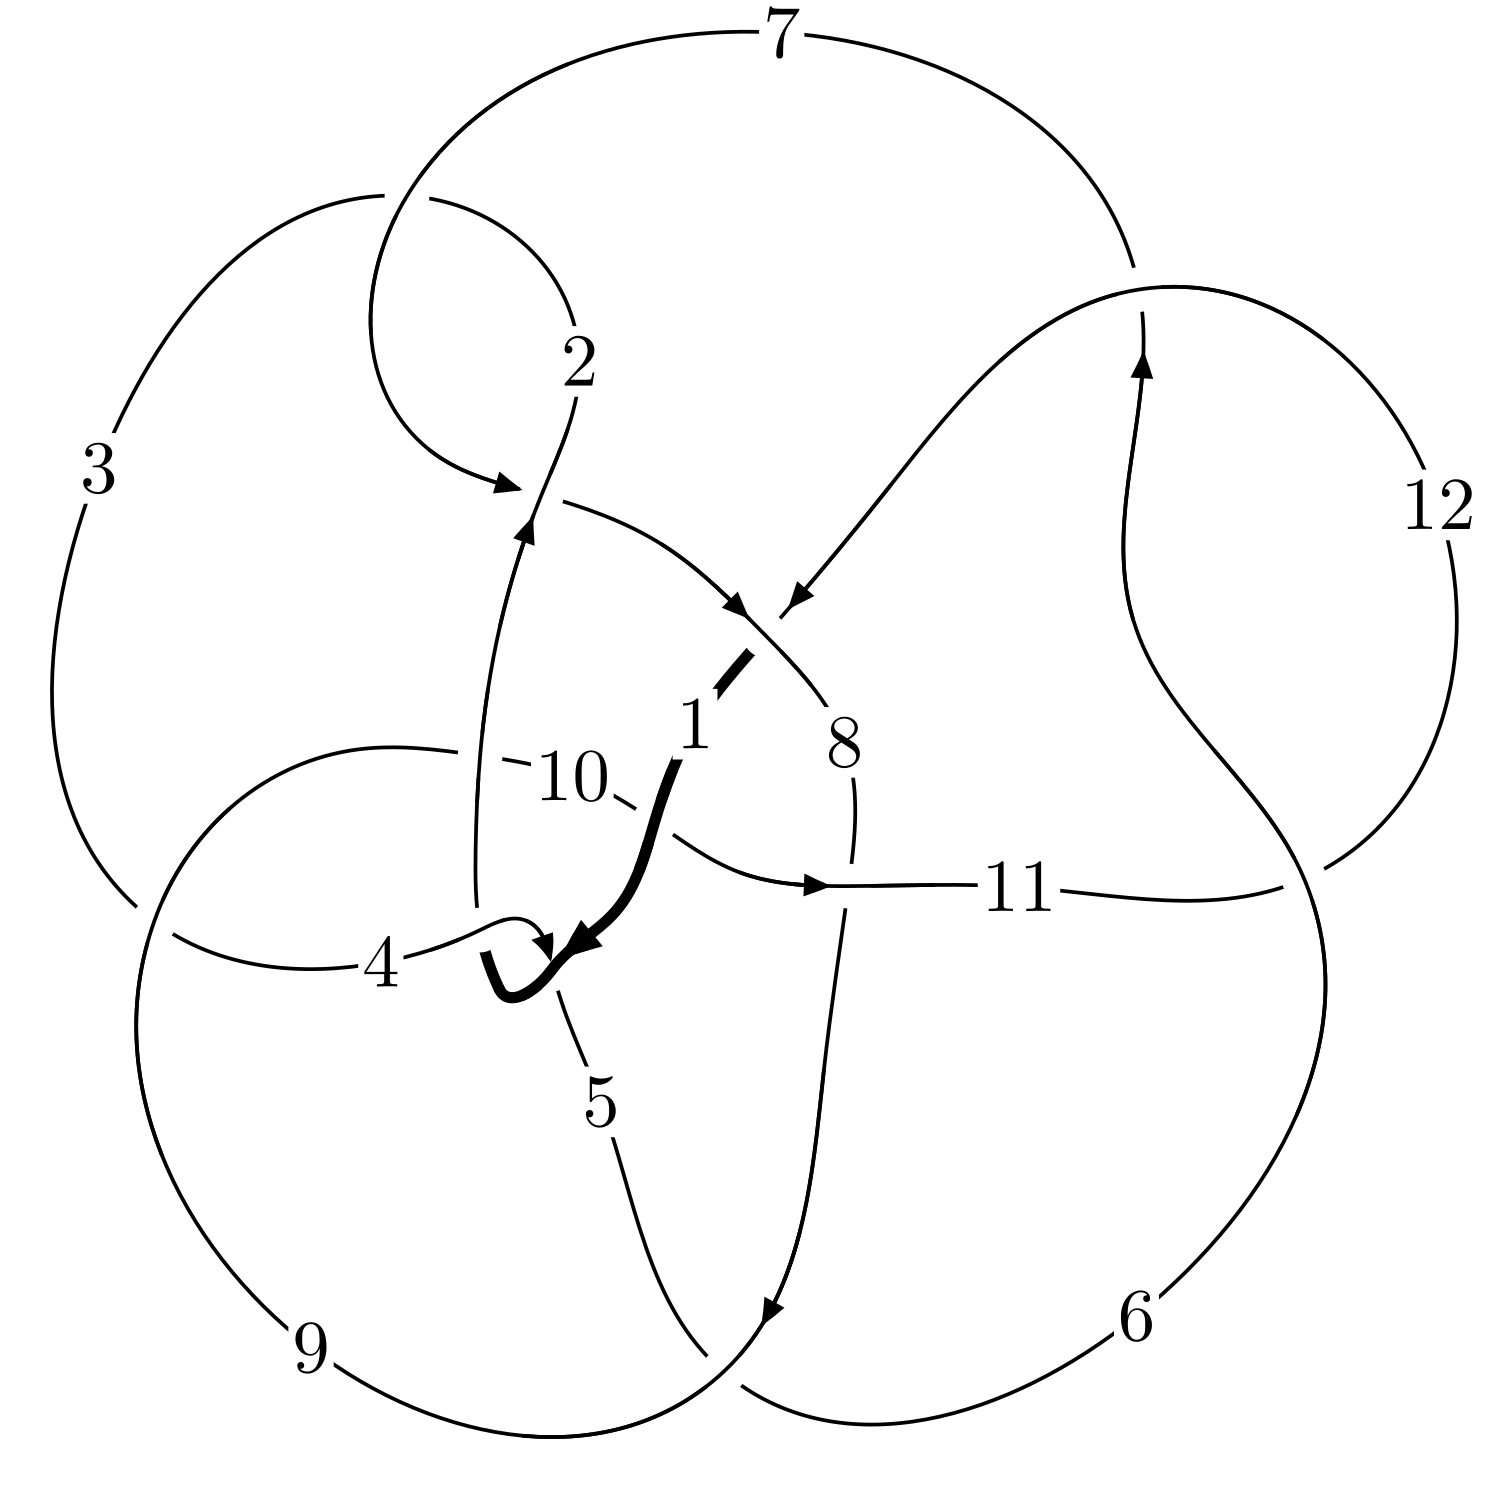
\includegraphics[width=112pt]{../../../GIT/diagram.site/Diagrams/png/2947_12n_0858.png}\\
\ \ \ A knot diagram\footnotemark}&
\allowdisplaybreaks
\textbf{Linearized knot diagam} \\
\cline{2-2}
 &
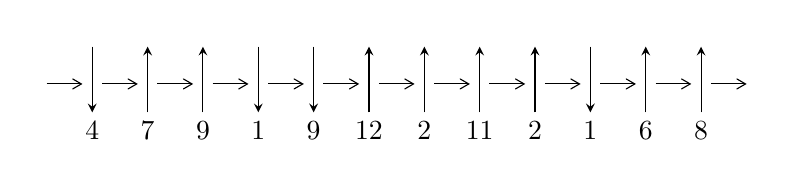
\begin{tikzpicture}[x=20pt, y=17pt]
	% nodes
	\node (C0) at (0, 0) {};
	\node (C1) at (1, 0) {};
	\node (C1U) at (1, +1) {};
	\node (C1D) at (1, -1) {4};

	\node (C2) at (2, 0) {};
	\node (C2U) at (2, +1) {};
	\node (C2D) at (2, -1) {7};

	\node (C3) at (3, 0) {};
	\node (C3U) at (3, +1) {};
	\node (C3D) at (3, -1) {9};

	\node (C4) at (4, 0) {};
	\node (C4U) at (4, +1) {};
	\node (C4D) at (4, -1) {1};

	\node (C5) at (5, 0) {};
	\node (C5U) at (5, +1) {};
	\node (C5D) at (5, -1) {9};

	\node (C6) at (6, 0) {};
	\node (C6U) at (6, +1) {};
	\node (C6D) at (6, -1) {12};

	\node (C7) at (7, 0) {};
	\node (C7U) at (7, +1) {};
	\node (C7D) at (7, -1) {2};

	\node (C8) at (8, 0) {};
	\node (C8U) at (8, +1) {};
	\node (C8D) at (8, -1) {11};

	\node (C9) at (9, 0) {};
	\node (C9U) at (9, +1) {};
	\node (C9D) at (9, -1) {2};

	\node (C10) at (10, 0) {};
	\node (C10U) at (10, +1) {};
	\node (C10D) at (10, -1) {1};

	\node (C11) at (11, 0) {};
	\node (C11U) at (11, +1) {};
	\node (C11D) at (11, -1) {6};

	\node (C12) at (12, 0) {};
	\node (C12U) at (12, +1) {};
	\node (C12D) at (12, -1) {8};
	\node (C13) at (13, 0) {};

	% arrows
	\draw[->,>={angle 60}]
	(C0) edge (C1) (C1) edge (C2) (C2) edge (C3) (C3) edge (C4) (C4) edge (C5) (C5) edge (C6) (C6) edge (C7) (C7) edge (C8) (C8) edge (C9) (C9) edge (C10) (C10) edge (C11) (C11) edge (C12) (C12) edge (C13) ;	\draw[->,>=stealth]
	(C1U) edge (C1D) (C2D) edge (C2U) (C3D) edge (C3U) (C4U) edge (C4D) (C5U) edge (C5D) (C6D) edge (C6U) (C7D) edge (C7U) (C8D) edge (C8U) (C9D) edge (C9U) (C10U) edge (C10D) (C11D) edge (C11U) (C12D) edge (C12U) ;
	\end{tikzpicture} \\
\hhline{~~} \\& 
\textbf{Solving Sequence} \\ \cline{2-2} 
 &
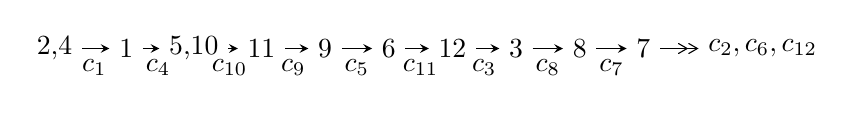
\begin{tikzpicture}[x=23pt, y=7pt]
	% node
	\node (A0) at (-1/8, 0) {2,4};
	\node (A1) at (1, 0) {1};
	\node (A2) at (33/16, 0) {5,10};
	\node (A3) at (25/8, 0) {11};
	\node (A4) at (33/8, 0) {9};
	\node (A5) at (41/8, 0) {6};
	\node (A6) at (49/8, 0) {12};
	\node (A7) at (57/8, 0) {3};
	\node (A8) at (65/8, 0) {8};
	\node (A9) at (73/8, 0) {7};
	\node (C1) at (1/2, -1) {$c_{1}$};
	\node (C2) at (3/2, -1) {$c_{4}$};
	\node (C3) at (21/8, -1) {$c_{10}$};
	\node (C4) at (29/8, -1) {$c_{9}$};
	\node (C5) at (37/8, -1) {$c_{5}$};
	\node (C6) at (45/8, -1) {$c_{11}$};
	\node (C7) at (53/8, -1) {$c_{3}$};
	\node (C8) at (61/8, -1) {$c_{8}$};
	\node (C9) at (69/8, -1) {$c_{7}$};
	\node (A10) at (11, 0) {$c_{2},c_{6},c_{12}$};

	% edge
	\draw[->,>=stealth]	
	(A0) edge (A1) (A1) edge (A2) (A2) edge (A3) (A3) edge (A4) (A4) edge (A5) (A5) edge (A6) (A6) edge (A7) (A7) edge (A8) (A8) edge (A9) ;
	\draw[->>,>={angle 60}]	
	(A9) edge (A10);
\end{tikzpicture} \\ 

\end{tabular} \\

\footnotetext{
The image of knot diagram is generated by the software ``\textbf{Draw programme}" developed by Andrew Bartholomew(\url{http://www.layer8.co.uk/maths/draw/index.htm\#Running-draw}), where we modified some parts for our purpose(\url{https://github.com/CATsTAILs/LinksPainter}).
}\phantom \\ \newline 
\centering \textbf{Ideals for irreducible components\footnotemark of $X_{\text{par}}$} 
 
\begin{align*}
I^u_{1}&=\langle 
-1.03636\times10^{222} u^{84}-3.95825\times10^{222} u^{83}+\cdots+1.02307\times10^{222} b-2.68730\times10^{221},\\
\phantom{I^u_{1}}&\phantom{= \langle  }-1.33652\times10^{222} u^{84}-4.40227\times10^{222} u^{83}+\cdots+3.06922\times10^{222} a-2.90267\times10^{223},\\
\phantom{I^u_{1}}&\phantom{= \langle  }u^{85}+4 u^{84}+\cdots+2 u+1\rangle \\
I^u_{2}&=\langle 
-2.67401\times10^{19} u^{27}+1.56488\times10^{20} u^{26}+\cdots+1.03296\times10^{19} b+9.72270\times10^{16},\\
\phantom{I^u_{2}}&\phantom{= \langle  }-2.83742\times10^{19} u^{27}+1.86866\times10^{20} u^{26}+\cdots+1.03296\times10^{19} a+1.15270\times10^{20},\;u^{28}-6 u^{27}+\cdots-5 u+1\rangle \\
I^u_{3}&=\langle 
b,\;a- u+1,\;u^2- u+1\rangle \\
\\
\end{align*}
\raggedright * 3 irreducible components of $\dim_{\mathbb{C}}=0$, with total 115 representations.\\
\footnotetext{All coefficients of polynomials are rational numbers. But the coefficients are sometimes approximated in decimal forms when there is not enough margin.}
\newpage
\renewcommand{\arraystretch}{1}
\centering \section*{I. $I^u_{1}= \langle -1.04\times10^{222} u^{84}-3.96\times10^{222} u^{83}+\cdots+1.02\times10^{222} b-2.69\times10^{221},\;-1.34\times10^{222} u^{84}-4.40\times10^{222} u^{83}+\cdots+3.07\times10^{222} a-2.90\times10^{223},\;u^{85}+4 u^{84}+\cdots+2 u+1 \rangle$}
\flushleft \textbf{(i) Arc colorings}\\
\begin{tabular}{m{7pt} m{180pt} m{7pt} m{180pt} }
\flushright $a_{2}=$&$\begin{pmatrix}1\\0\end{pmatrix}$ \\
\flushright $a_{4}=$&$\begin{pmatrix}0\\u\end{pmatrix}$ \\
\flushright $a_{1}=$&$\begin{pmatrix}1\\- u^2\end{pmatrix}$ \\
\flushright $a_{5}=$&$\begin{pmatrix}- u\\u^3+u\end{pmatrix}$ \\
\flushright $a_{10}=$&$\begin{pmatrix}0.435460 u^{84}+1.43433 u^{83}+\cdots-57.4184 u+9.45737\\1.01299 u^{84}+3.86898 u^{83}+\cdots+18.3676 u+0.262670\end{pmatrix}$ \\
\flushright $a_{11}=$&$\begin{pmatrix}-0.0186202 u^{84}-0.424498 u^{83}+\cdots-75.9656 u+8.88719\\0.905660 u^{84}+3.44358 u^{83}+\cdots+17.8285 u+0.220165\end{pmatrix}$ \\
\flushright $a_{9}=$&$\begin{pmatrix}-0.577528 u^{84}-2.43465 u^{83}+\cdots-75.7860 u+9.19470\\1.01299 u^{84}+3.86898 u^{83}+\cdots+18.3676 u+0.262670\end{pmatrix}$ \\
\flushright $a_{6}=$&$\begin{pmatrix}-0.342675 u^{84}-1.51095 u^{83}+\cdots-91.5089 u-14.8953\\-0.120732 u^{84}-0.834502 u^{83}+\cdots-5.90626 u+0.893350\end{pmatrix}$ \\
\flushright $a_{12}=$&$\begin{pmatrix}0.303518 u^{84}+0.747086 u^{83}+\cdots+102.130 u+17.1171\\0.499714 u^{84}+1.68173 u^{83}+\cdots+5.70936 u-2.24895\end{pmatrix}$ \\
\flushright $a_{3}=$&$\begin{pmatrix}0.279580 u^{84}+0.737945 u^{83}+\cdots-83.3181 u-17.0118\\-0.216374 u^{84}-0.998041 u^{83}+\cdots-6.67199 u+1.73603\end{pmatrix}$ \\
\flushright $a_{8}=$&$\begin{pmatrix}-2.00860 u^{84}-8.08594 u^{83}+\cdots-109.439 u+4.86586\\0.228258 u^{84}+1.23880 u^{83}+\cdots+16.5717 u+1.16566\end{pmatrix}$ \\
\flushright $a_{7}=$&$\begin{pmatrix}-2.23686 u^{84}-9.32474 u^{83}+\cdots-126.011 u+3.70020\\0.228258 u^{84}+1.23880 u^{83}+\cdots+16.5717 u+1.16566\end{pmatrix}$\\&\end{tabular}
\flushleft \textbf{(ii) Obstruction class $= -1$}\\~\\
\flushleft \textbf{(iii) Cusp Shapes $= -5.33059 u^{84}-22.7759 u^{83}+\cdots-48.3401 u-9.30996$}\\~\\
\newpage\renewcommand{\arraystretch}{1}
\flushleft \textbf{(iv) u-Polynomials at the component}\newline \\
\begin{tabular}{m{50pt}|m{274pt}}
Crossings & \hspace{64pt}u-Polynomials at each crossing \\
\hline $$\begin{aligned}c_{1},c_{4}\end{aligned}$$&$\begin{aligned}
&u^{85}-4 u^{84}+\cdots+2 u-1
\end{aligned}$\\
\hline $$\begin{aligned}c_{2},c_{7}\end{aligned}$$&$\begin{aligned}
&u^{85}+30 u^{83}+\cdots+26 u-1
\end{aligned}$\\
\hline $$\begin{aligned}c_{3}\end{aligned}$$&$\begin{aligned}
&u^{85}+u^{84}+\cdots-8586859 u-7135679
\end{aligned}$\\
\hline $$\begin{aligned}c_{5}\end{aligned}$$&$\begin{aligned}
&u^{85}+10 u^{84}+\cdots+4292211 u-291526
\end{aligned}$\\
\hline $$\begin{aligned}c_{6},c_{11}\end{aligned}$$&$\begin{aligned}
&u^{85}+2 u^{84}+\cdots-564 u-172
\end{aligned}$\\
\hline $$\begin{aligned}c_{8}\end{aligned}$$&$\begin{aligned}
&u^{85}+u^{84}+\cdots+15 u+1
\end{aligned}$\\
\hline $$\begin{aligned}c_{9}\end{aligned}$$&$\begin{aligned}
&u^{85}-3 u^{84}+\cdots+5809196 u-707552
\end{aligned}$\\
\hline $$\begin{aligned}c_{10}\end{aligned}$$&$\begin{aligned}
&u^{85}-12 u^{84}+\cdots+63060030 u-7539289
\end{aligned}$\\
\hline $$\begin{aligned}c_{12}\end{aligned}$$&$\begin{aligned}
&u^{85}-3 u^{84}+\cdots-35799 u-3454
\end{aligned}$\\
\hline
\end{tabular}\\~\\
\newpage\renewcommand{\arraystretch}{1}
\flushleft \textbf{(v) Riley Polynomials at the component}\newline \\
\begin{tabular}{m{50pt}|m{274pt}}
Crossings & \hspace{64pt}Riley Polynomials at each crossing \\
\hline $$\begin{aligned}c_{1},c_{4}\end{aligned}$$&$\begin{aligned}
&y^{85}+18 y^{84}+\cdots-228 y-1
\end{aligned}$\\
\hline $$\begin{aligned}c_{2},c_{7}\end{aligned}$$&$\begin{aligned}
&y^{85}+60 y^{84}+\cdots-140 y-1
\end{aligned}$\\
\hline $$\begin{aligned}c_{3}\end{aligned}$$&$\begin{aligned}
&y^{85}+75 y^{84}+\cdots-496895527067841 y-50917914791041
\end{aligned}$\\
\hline $$\begin{aligned}c_{5}\end{aligned}$$&$\begin{aligned}
&y^{85}-38 y^{84}+\cdots+7819625711645 y-84987408676
\end{aligned}$\\
\hline $$\begin{aligned}c_{6},c_{11}\end{aligned}$$&$\begin{aligned}
&y^{85}-50 y^{84}+\cdots+783184 y-29584
\end{aligned}$\\
\hline $$\begin{aligned}c_{8}\end{aligned}$$&$\begin{aligned}
&y^{85}-15 y^{84}+\cdots-11 y-1
\end{aligned}$\\
\hline $$\begin{aligned}c_{9}\end{aligned}$$&$\begin{aligned}
&y^{85}+77 y^{84}+\cdots-9930483397744 y-500629832704
\end{aligned}$\\
\hline $$\begin{aligned}c_{10}\end{aligned}$$&$\begin{aligned}
&y^{85}-44 y^{84}+\cdots+214383869545346 y-56840878625521
\end{aligned}$\\
\hline $$\begin{aligned}c_{12}\end{aligned}$$&$\begin{aligned}
&y^{85}+17 y^{84}+\cdots-589394319 y-11930116
\end{aligned}$\\
\hline
\end{tabular}\\~\\
\newpage\flushleft \textbf{(vi) Complex Volumes and Cusp Shapes}
$$\begin{array}{c|c|c}  
\text{Solutions to }I^u_{1}& \I (\text{vol} + \sqrt{-1}CS) & \text{Cusp shape}\\
 \hline 
\begin{aligned}
u &= \phantom{-}0.998570 + 0.272294 I \\
a &= \phantom{-}0.475791 - 0.395407 I \\
b &= \phantom{-}0.032394 - 0.448924 I\end{aligned}
 & -1.43220 - 2.66932 I & \phantom{-0.000000 } 0 \\ \hline\begin{aligned}
u &= \phantom{-}0.998570 - 0.272294 I \\
a &= \phantom{-}0.475791 + 0.395407 I \\
b &= \phantom{-}0.032394 + 0.448924 I\end{aligned}
 & -1.43220 + 2.66932 I & \phantom{-0.000000 } 0 \\ \hline\begin{aligned}
u &= -0.078052 + 0.926381 I \\
a &= \phantom{-}1.92195 + 1.40477 I \\
b &= \phantom{-}0.773943 + 0.472131 I\end{aligned}
 & -0.217172 - 1.098890 I & \phantom{-0.000000 } 0 \\ \hline\begin{aligned}
u &= -0.078052 - 0.926381 I \\
a &= \phantom{-}1.92195 - 1.40477 I \\
b &= \phantom{-}0.773943 - 0.472131 I\end{aligned}
 & -0.217172 + 1.098890 I & \phantom{-0.000000 } 0 \\ \hline\begin{aligned}
u &= -0.981755 + 0.507072 I \\
a &= \phantom{-}0.196732 + 1.354770 I \\
b &= \phantom{-}0.04903 + 2.35138 I\end{aligned}
 & -3.61008 + 5.45903 I & \phantom{-0.000000 } 0 \\ \hline\begin{aligned}
u &= -0.981755 - 0.507072 I \\
a &= \phantom{-}0.196732 - 1.354770 I \\
b &= \phantom{-}0.04903 - 2.35138 I\end{aligned}
 & -3.61008 - 5.45903 I & \phantom{-0.000000 } 0 \\ \hline\begin{aligned}
u &= \phantom{-}0.476670 + 1.051240 I \\
a &= -0.325982 + 0.333193 I \\
b &= -0.425103 - 0.302685 I\end{aligned}
 & \phantom{-}0.96688 - 5.57781 I & \phantom{-0.000000 } 0 \\ \hline\begin{aligned}
u &= \phantom{-}0.476670 - 1.051240 I \\
a &= -0.325982 - 0.333193 I \\
b &= -0.425103 + 0.302685 I\end{aligned}
 & \phantom{-}0.96688 + 5.57781 I & \phantom{-0.000000 } 0 \\ \hline\begin{aligned}
u &= \phantom{-}0.668482 + 0.952846 I \\
a &= \phantom{-}0.945938 - 0.449100 I \\
b &= \phantom{-}0.277270 - 0.487750 I\end{aligned}
 & \phantom{-}0.47254 - 2.58298 I & \phantom{-0.000000 } 0 \\ \hline\begin{aligned}
u &= \phantom{-}0.668482 - 0.952846 I \\
a &= \phantom{-}0.945938 + 0.449100 I \\
b &= \phantom{-}0.277270 + 0.487750 I\end{aligned}
 & \phantom{-}0.47254 + 2.58298 I & \phantom{-0.000000 } 0\\
 \hline 
 \end{array}$$\newpage$$\begin{array}{c|c|c}  
\text{Solutions to }I^u_{1}& \I (\text{vol} + \sqrt{-1}CS) & \text{Cusp shape}\\
 \hline 
\begin{aligned}
u &= \phantom{-}0.191158 + 0.810743 I \\
a &= \phantom{-}0.399071 - 0.163081 I \\
b &= \phantom{-}1.13355 - 1.50881 I\end{aligned}
 & \phantom{-}0.59219 + 4.00643 I & \phantom{-}9.81408 - 1.58250 I \\ \hline\begin{aligned}
u &= \phantom{-}0.191158 - 0.810743 I \\
a &= \phantom{-}0.399071 + 0.163081 I \\
b &= \phantom{-}1.13355 + 1.50881 I\end{aligned}
 & \phantom{-}0.59219 - 4.00643 I & \phantom{-}9.81408 + 1.58250 I \\ \hline\begin{aligned}
u &= \phantom{-}0.920774 + 0.721880 I \\
a &= -1.023550 + 0.281002 I \\
b &= -0.67699 + 1.48386 I\end{aligned}
 & -4.32440 - 1.41643 I & \phantom{-0.000000 } 0 \\ \hline\begin{aligned}
u &= \phantom{-}0.920774 - 0.721880 I \\
a &= -1.023550 - 0.281002 I \\
b &= -0.67699 - 1.48386 I\end{aligned}
 & -4.32440 + 1.41643 I & \phantom{-0.000000 } 0 \\ \hline\begin{aligned}
u &= -0.114215 + 0.796267 I \\
a &= -1.47054 + 0.01938 I \\
b &= -0.738208 + 0.689403 I\end{aligned}
 & \phantom{-}6.75942 - 3.17501 I & \phantom{-}7.34012 + 8.97310 I \\ \hline\begin{aligned}
u &= -0.114215 - 0.796267 I \\
a &= -1.47054 - 0.01938 I \\
b &= -0.738208 - 0.689403 I\end{aligned}
 & \phantom{-}6.75942 + 3.17501 I & \phantom{-}7.34012 - 8.97310 I \\ \hline\begin{aligned}
u &= -0.289881 + 0.745166 I \\
a &= \phantom{-}1.140080 - 0.820492 I \\
b &= \phantom{-}1.57828 + 0.62135 I\end{aligned}
 & \phantom{-}6.89613 + 1.55029 I & \phantom{-}8.65169 - 1.88696 I \\ \hline\begin{aligned}
u &= -0.289881 - 0.745166 I \\
a &= \phantom{-}1.140080 + 0.820492 I \\
b &= \phantom{-}1.57828 - 0.62135 I\end{aligned}
 & \phantom{-}6.89613 - 1.55029 I & \phantom{-}8.65169 + 1.88696 I \\ \hline\begin{aligned}
u &= \phantom{-}0.736997 + 0.309730 I \\
a &= -1.003550 - 0.492868 I \\
b &= -1.219120 + 0.187207 I\end{aligned}
 & -3.36308 - 1.67385 I & -3.09379 + 4.70980 I \\ \hline\begin{aligned}
u &= \phantom{-}0.736997 - 0.309730 I \\
a &= -1.003550 + 0.492868 I \\
b &= -1.219120 - 0.187207 I\end{aligned}
 & -3.36308 + 1.67385 I & -3.09379 - 4.70980 I\\
 \hline 
 \end{array}$$\newpage$$\begin{array}{c|c|c}  
\text{Solutions to }I^u_{1}& \I (\text{vol} + \sqrt{-1}CS) & \text{Cusp shape}\\
 \hline 
\begin{aligned}
u &= -0.784929 + 0.921642 I \\
a &= -0.819247 - 1.130810 I \\
b &= \phantom{-}0.36426 - 1.68162 I\end{aligned}
 & -6.55646 - 2.64119 I & \phantom{-0.000000 } 0 \\ \hline\begin{aligned}
u &= -0.784929 - 0.921642 I \\
a &= -0.819247 + 1.130810 I \\
b &= \phantom{-}0.36426 + 1.68162 I\end{aligned}
 & -6.55646 + 2.64119 I & \phantom{-0.000000 } 0 \\ \hline\begin{aligned}
u &= -1.007190 + 0.675787 I \\
a &= -1.327370 + 0.100127 I \\
b &= -0.324588 - 1.238780 I\end{aligned}
 & -5.94666 + 1.03450 I & \phantom{-0.000000 } 0 \\ \hline\begin{aligned}
u &= -1.007190 - 0.675787 I \\
a &= -1.327370 - 0.100127 I \\
b &= -0.324588 + 1.238780 I\end{aligned}
 & -5.94666 - 1.03450 I & \phantom{-0.000000 } 0 \\ \hline\begin{aligned}
u &= \phantom{-}1.111950 + 0.502144 I \\
a &= -0.682297 - 0.061208 I \\
b &= -0.457963 + 0.733480 I\end{aligned}
 & -3.52529 - 1.34010 I & \phantom{-0.000000 } 0 \\ \hline\begin{aligned}
u &= \phantom{-}1.111950 - 0.502144 I \\
a &= -0.682297 + 0.061208 I \\
b &= -0.457963 - 0.733480 I\end{aligned}
 & -3.52529 + 1.34010 I & \phantom{-0.000000 } 0 \\ \hline\begin{aligned}
u &= -0.840950 + 0.891035 I \\
a &= -1.51043 - 0.31627 I \\
b &= -1.00700 - 1.77133 I\end{aligned}
 & -6.68939 + 8.75504 I & \phantom{-0.000000 } 0 \\ \hline\begin{aligned}
u &= -0.840950 - 0.891035 I \\
a &= -1.51043 + 0.31627 I \\
b &= -1.00700 + 1.77133 I\end{aligned}
 & -6.68939 - 8.75504 I & \phantom{-0.000000 } 0 \\ \hline\begin{aligned}
u &= \phantom{-}0.528662 + 0.545614 I \\
a &= \phantom{-}1.47316 - 2.31272 I \\
b &= -0.688160 - 0.114075 I\end{aligned}
 & -0.66682 - 6.93179 I & \phantom{-}4.00000 + 11.91492 I \\ \hline\begin{aligned}
u &= \phantom{-}0.528662 - 0.545614 I \\
a &= \phantom{-}1.47316 + 2.31272 I \\
b &= -0.688160 + 0.114075 I\end{aligned}
 & -0.66682 + 6.93179 I & \phantom{-}4.00000 - 11.91492 I\\
 \hline 
 \end{array}$$\newpage$$\begin{array}{c|c|c}  
\text{Solutions to }I^u_{1}& \I (\text{vol} + \sqrt{-1}CS) & \text{Cusp shape}\\
 \hline 
\begin{aligned}
u &= -0.064801 + 1.255050 I \\
a &= -0.327089 + 0.427849 I \\
b &= \phantom{-}0.094931 + 0.511084 I\end{aligned}
 & \phantom{-}5.65951 + 1.98333 I & \phantom{-0.000000 } 0 \\ \hline\begin{aligned}
u &= -0.064801 - 1.255050 I \\
a &= -0.327089 - 0.427849 I \\
b &= \phantom{-}0.094931 - 0.511084 I\end{aligned}
 & \phantom{-}5.65951 - 1.98333 I & \phantom{-0.000000 } 0 \\ \hline\begin{aligned}
u &= \phantom{-}0.995122 + 0.770188 I \\
a &= \phantom{-}0.941647 - 0.500048 I \\
b &= \phantom{-}0.14802 - 1.67413 I\end{aligned}
 & -2.68266 + 2.97750 I & \phantom{-0.000000 } 0 \\ \hline\begin{aligned}
u &= \phantom{-}0.995122 - 0.770188 I \\
a &= \phantom{-}0.941647 + 0.500048 I \\
b &= \phantom{-}0.14802 + 1.67413 I\end{aligned}
 & -2.68266 - 2.97750 I & \phantom{-0.000000 } 0 \\ \hline\begin{aligned}
u &= -0.117101 + 0.723899 I \\
a &= -0.793624 - 0.270354 I \\
b &= -1.35991 + 0.87928 I\end{aligned}
 & -0.655020 + 1.237870 I & \phantom{-}10.88550 - 2.57862 I \\ \hline\begin{aligned}
u &= -0.117101 - 0.723899 I \\
a &= -0.793624 + 0.270354 I \\
b &= -1.35991 - 0.87928 I\end{aligned}
 & -0.655020 - 1.237870 I & \phantom{-}10.88550 + 2.57862 I \\ \hline\begin{aligned}
u &= -0.443214 + 0.560209 I \\
a &= \phantom{-}1.84470 + 0.04018 I \\
b &= \phantom{-}0.881631 - 0.377895 I\end{aligned}
 & \phantom{-}5.65422 + 5.51636 I & \phantom{-}16.4245 + 6.0413 I \\ \hline\begin{aligned}
u &= -0.443214 - 0.560209 I \\
a &= \phantom{-}1.84470 - 0.04018 I \\
b &= \phantom{-}0.881631 + 0.377895 I\end{aligned}
 & \phantom{-}5.65422 - 5.51636 I & \phantom{-}16.4245 - 6.0413 I \\ \hline\begin{aligned}
u &= -0.926014 + 0.904807 I \\
a &= \phantom{-}1.315410 + 0.385771 I \\
b &= \phantom{-}0.51296 + 1.85233 I\end{aligned}
 & -8.99774 + 4.10945 I & \phantom{-0.000000 } 0 \\ \hline\begin{aligned}
u &= -0.926014 - 0.904807 I \\
a &= \phantom{-}1.315410 - 0.385771 I \\
b &= \phantom{-}0.51296 - 1.85233 I\end{aligned}
 & -8.99774 - 4.10945 I & \phantom{-0.000000 } 0\\
 \hline 
 \end{array}$$\newpage$$\begin{array}{c|c|c}  
\text{Solutions to }I^u_{1}& \I (\text{vol} + \sqrt{-1}CS) & \text{Cusp shape}\\
 \hline 
\begin{aligned}
u &= \phantom{-}1.016570 + 0.802307 I \\
a &= \phantom{-}0.501441 - 0.416278 I \\
b &= \phantom{-}0.370374 - 1.209920 I\end{aligned}
 & -0.70125 - 3.83022 I & \phantom{-0.000000 } 0 \\ \hline\begin{aligned}
u &= \phantom{-}1.016570 - 0.802307 I \\
a &= \phantom{-}0.501441 + 0.416278 I \\
b &= \phantom{-}0.370374 + 1.209920 I\end{aligned}
 & -0.70125 + 3.83022 I & \phantom{-0.000000 } 0 \\ \hline\begin{aligned}
u &= \phantom{-}0.393407 + 1.253670 I \\
a &= \phantom{-}0.816751 - 0.028019 I \\
b &= \phantom{-}0.380543 - 0.236715 I\end{aligned}
 & \phantom{-}0.87862 - 2.40445 I & \phantom{-0.000000 } 0 \\ \hline\begin{aligned}
u &= \phantom{-}0.393407 - 1.253670 I \\
a &= \phantom{-}0.816751 + 0.028019 I \\
b &= \phantom{-}0.380543 + 0.236715 I\end{aligned}
 & \phantom{-}0.87862 + 2.40445 I & \phantom{-0.000000 } 0 \\ \hline\begin{aligned}
u &= -0.873771 + 0.982867 I \\
a &= \phantom{-}0.932327 + 0.814540 I \\
b &= -0.11560 + 1.83982 I\end{aligned}
 & -8.72930 + 2.55502 I & \phantom{-0.000000 } 0 \\ \hline\begin{aligned}
u &= -0.873771 - 0.982867 I \\
a &= \phantom{-}0.932327 - 0.814540 I \\
b &= -0.11560 - 1.83982 I\end{aligned}
 & -8.72930 - 2.55502 I & \phantom{-0.000000 } 0 \\ \hline\begin{aligned}
u &= -0.322301 + 0.597684 I \\
a &= -0.98727 + 2.66264 I \\
b &= -1.275690 - 0.115283 I\end{aligned}
 & \phantom{-}6.34439 + 0.92935 I & \phantom{-}20.3887 - 11.8228 I \\ \hline\begin{aligned}
u &= -0.322301 - 0.597684 I \\
a &= -0.98727 - 2.66264 I \\
b &= -1.275690 + 0.115283 I\end{aligned}
 & \phantom{-}6.34439 - 0.92935 I & \phantom{-}20.3887 + 11.8228 I \\ \hline\begin{aligned}
u &= \phantom{-}0.012130 + 0.671137 I \\
a &= -3.61616 - 1.88171 I \\
b &= -1.160720 - 0.362352 I\end{aligned}
 & \phantom{-}1.07314 + 5.28326 I & \phantom{-}12.72232 - 3.52720 I \\ \hline\begin{aligned}
u &= \phantom{-}0.012130 - 0.671137 I \\
a &= -3.61616 + 1.88171 I \\
b &= -1.160720 + 0.362352 I\end{aligned}
 & \phantom{-}1.07314 - 5.28326 I & \phantom{-}12.72232 + 3.52720 I\\
 \hline 
 \end{array}$$\newpage$$\begin{array}{c|c|c}  
\text{Solutions to }I^u_{1}& \I (\text{vol} + \sqrt{-1}CS) & \text{Cusp shape}\\
 \hline 
\begin{aligned}
u &= \phantom{-}0.320917 + 0.576461 I \\
a &= \phantom{-}0.44228 + 2.73702 I \\
b &= \phantom{-}0.595528 - 0.251518 I\end{aligned}
 & -1.32168 - 2.14852 I & \phantom{-}5.67361 + 6.10919 I \\ \hline\begin{aligned}
u &= \phantom{-}0.320917 - 0.576461 I \\
a &= \phantom{-}0.44228 - 2.73702 I \\
b &= \phantom{-}0.595528 + 0.251518 I\end{aligned}
 & -1.32168 + 2.14852 I & \phantom{-}5.67361 - 6.10919 I \\ \hline\begin{aligned}
u &= \phantom{-}0.792598 + 1.092070 I \\
a &= -0.934721 + 0.937326 I \\
b &= -0.06898 + 1.54472 I\end{aligned}
 & -3.16562 - 4.95912 I & \phantom{-0.000000 } 0 \\ \hline\begin{aligned}
u &= \phantom{-}0.792598 - 1.092070 I \\
a &= -0.934721 - 0.937326 I \\
b &= -0.06898 - 1.54472 I\end{aligned}
 & -3.16562 + 4.95912 I & \phantom{-0.000000 } 0 \\ \hline\begin{aligned}
u &= -1.068700 + 0.849855 I \\
a &= -0.730782 - 0.967920 I \\
b &= \phantom{-}0.05722 - 1.85054 I\end{aligned}
 & -10.13780 - 3.22951 I & \phantom{-0.000000 } 0 \\ \hline\begin{aligned}
u &= -1.068700 - 0.849855 I \\
a &= -0.730782 + 0.967920 I \\
b &= \phantom{-}0.05722 + 1.85054 I\end{aligned}
 & -10.13780 + 3.22951 I & \phantom{-0.000000 } 0 \\ \hline\begin{aligned}
u &= \phantom{-}0.306326 + 0.542199 I \\
a &= \phantom{-}1.96796 + 0.29112 I \\
b &= \phantom{-}2.60639 - 0.46014 I\end{aligned}
 & \phantom{-}0.38559 - 6.54347 I & \phantom{-}7.3888 + 12.6144 I \\ \hline\begin{aligned}
u &= \phantom{-}0.306326 - 0.542199 I \\
a &= \phantom{-}1.96796 - 0.29112 I \\
b &= \phantom{-}2.60639 + 0.46014 I\end{aligned}
 & \phantom{-}0.38559 + 6.54347 I & \phantom{-}7.3888 - 12.6144 I \\ \hline\begin{aligned}
u &= \phantom{-}0.854442 + 1.081810 I \\
a &= \phantom{-}1.21765 - 0.74563 I \\
b &= \phantom{-}0.39692 - 1.85331 I\end{aligned}
 & -1.70018 - 9.75286 I & \phantom{-0.000000 } 0 \\ \hline\begin{aligned}
u &= \phantom{-}0.854442 - 1.081810 I \\
a &= \phantom{-}1.21765 + 0.74563 I \\
b &= \phantom{-}0.39692 + 1.85331 I\end{aligned}
 & -1.70018 + 9.75286 I & \phantom{-0.000000 } 0\\
 \hline 
 \end{array}$$\newpage$$\begin{array}{c|c|c}  
\text{Solutions to }I^u_{1}& \I (\text{vol} + \sqrt{-1}CS) & \text{Cusp shape}\\
 \hline 
\begin{aligned}
u &= -1.103910 + 0.843065 I \\
a &= \phantom{-}0.694324 + 0.843846 I \\
b &= -0.27662 + 1.65789 I\end{aligned}
 & -6.92146 - 10.17200 I & \phantom{-0.000000 } 0 \\ \hline\begin{aligned}
u &= -1.103910 - 0.843065 I \\
a &= \phantom{-}0.694324 - 0.843846 I \\
b &= -0.27662 - 1.65789 I\end{aligned}
 & -6.92146 + 10.17200 I & \phantom{-0.000000 } 0 \\ \hline\begin{aligned}
u &= \phantom{-}0.892642 + 1.067060 I \\
a &= \phantom{-}0.938403 - 0.382310 I \\
b &= \phantom{-}0.697204 - 1.065550 I\end{aligned}
 & \phantom{-}0.08231 - 3.35812 I & \phantom{-0.000000 } 0 \\ \hline\begin{aligned}
u &= \phantom{-}0.892642 - 1.067060 I \\
a &= \phantom{-}0.938403 + 0.382310 I \\
b &= \phantom{-}0.697204 + 1.065550 I\end{aligned}
 & \phantom{-}0.08231 + 3.35812 I & \phantom{-0.000000 } 0 \\ \hline\begin{aligned}
u &= -0.343571 + 0.493749 I \\
a &= -1.63279 - 0.47457 I \\
b &= -0.610765 + 0.376866 I\end{aligned}
 & \phantom{-}0.27736 + 2.37656 I & \phantom{-}5.87909 - 3.02757 I \\ \hline\begin{aligned}
u &= -0.343571 - 0.493749 I \\
a &= -1.63279 + 0.47457 I \\
b &= -0.610765 - 0.376866 I\end{aligned}
 & \phantom{-}0.27736 - 2.37656 I & \phantom{-}5.87909 + 3.02757 I \\ \hline\begin{aligned}
u &= -0.92042 + 1.08713 I \\
a &= -1.44989 - 0.76383 I \\
b &= -0.72095 - 1.86483 I\end{aligned}
 & -9.35077 + 10.45160 I & \phantom{-0.000000 } 0 \\ \hline\begin{aligned}
u &= -0.92042 - 1.08713 I \\
a &= -1.44989 + 0.76383 I \\
b &= -0.72095 + 1.86483 I\end{aligned}
 & -9.35077 - 10.45160 I & \phantom{-0.000000 } 0 \\ \hline\begin{aligned}
u &= -0.99205 + 1.02772 I \\
a &= \phantom{-}1.22952 + 1.05529 I \\
b &= \phantom{-}0.60550 + 1.78764 I\end{aligned}
 & -1.88830 + 3.70194 I & \phantom{-0.000000 } 0 \\ \hline\begin{aligned}
u &= -0.99205 - 1.02772 I \\
a &= \phantom{-}1.22952 - 1.05529 I \\
b &= \phantom{-}0.60550 - 1.78764 I\end{aligned}
 & -1.88830 - 3.70194 I & \phantom{-0.000000 } 0\\
 \hline 
 \end{array}$$\newpage$$\begin{array}{c|c|c}  
\text{Solutions to }I^u_{1}& \I (\text{vol} + \sqrt{-1}CS) & \text{Cusp shape}\\
 \hline 
\begin{aligned}
u &= -0.082020 + 0.555614 I \\
a &= \phantom{-}1.56239 + 0.33583 I \\
b &= \phantom{-}0.472829 - 0.368700 I\end{aligned}
 & \phantom{-}0.944298 - 0.816678 I & \phantom{-}7.73863 + 4.64902 I \\ \hline\begin{aligned}
u &= -0.082020 - 0.555614 I \\
a &= \phantom{-}1.56239 - 0.33583 I \\
b &= \phantom{-}0.472829 + 0.368700 I\end{aligned}
 & \phantom{-}0.944298 + 0.816678 I & \phantom{-}7.73863 - 4.64902 I \\ \hline\begin{aligned}
u &= -0.92506 + 1.10315 I \\
a &= \phantom{-}1.39631 + 0.61370 I \\
b &= \phantom{-}0.83273 + 1.89767 I\end{aligned}
 & -6.0450 + 17.5019 I & \phantom{-0.000000 } 0 \\ \hline\begin{aligned}
u &= -0.92506 - 1.10315 I \\
a &= \phantom{-}1.39631 - 0.61370 I \\
b &= \phantom{-}0.83273 - 1.89767 I\end{aligned}
 & -6.0450 - 17.5019 I & \phantom{-0.000000 } 0 \\ \hline\begin{aligned}
u &= -0.86980 + 1.18983 I \\
a &= -0.546302 - 0.583978 I \\
b &= \phantom{-}0.00460 - 1.61732 I\end{aligned}
 & -4.35655 + 5.88159 I & \phantom{-0.000000 } 0 \\ \hline\begin{aligned}
u &= -0.86980 - 1.18983 I \\
a &= -0.546302 + 0.583978 I \\
b &= \phantom{-}0.00460 + 1.61732 I\end{aligned}
 & -4.35655 - 5.88159 I & \phantom{-0.000000 } 0 \\ \hline\begin{aligned}
u &= -1.14823 + 0.94306 I \\
a &= \phantom{-}0.890564 + 0.131393 I \\
b &= \phantom{-}0.15158 + 1.57372 I\end{aligned}
 & -7.94495 + 4.03692 I & \phantom{-0.000000 } 0 \\ \hline\begin{aligned}
u &= -1.14823 - 0.94306 I \\
a &= \phantom{-}0.890564 - 0.131393 I \\
b &= \phantom{-}0.15158 - 1.57372 I\end{aligned}
 & -7.94495 - 4.03692 I & \phantom{-0.000000 } 0 \\ \hline\begin{aligned}
u &= -0.503477\phantom{ +0.000000I} \\
a &= \phantom{-}1.44168\phantom{ +0.000000I} \\
b &= \phantom{-}0.367391\phantom{ +0.000000I}\end{aligned}
 & \phantom{-}1.50635\phantom{ +0.000000I} & \phantom{-}7.56670\phantom{ +0.000000I} \\ \hline\begin{aligned}
u &= \phantom{-}0.94565 + 1.23775 I \\
a &= -0.651844 + 0.326553 I \\
b &= -0.437766 + 1.035920 I\end{aligned}
 & -1.43053 - 6.16651 I & \phantom{-0.000000 } 0\\
 \hline 
 \end{array}$$\newpage$$\begin{array}{c|c|c}  
\text{Solutions to }I^u_{1}& \I (\text{vol} + \sqrt{-1}CS) & \text{Cusp shape}\\
 \hline 
\begin{aligned}
u &= \phantom{-}0.94565 - 1.23775 I \\
a &= -0.651844 - 0.326553 I \\
b &= -0.437766 - 1.035920 I\end{aligned}
 & -1.43053 + 6.16651 I & \phantom{-0.000000 } 0 \\ \hline\begin{aligned}
u &= \phantom{-}0.38268 + 1.53582 I \\
a &= -0.201689 - 0.209453 I \\
b &= \phantom{-}0.120638 - 0.218357 I\end{aligned}
 & \phantom{-}4.55229 - 8.07421 I & \phantom{-0.000000 } 0 \\ \hline\begin{aligned}
u &= \phantom{-}0.38268 - 1.53582 I \\
a &= -0.201689 + 0.209453 I \\
b &= \phantom{-}0.120638 + 0.218357 I\end{aligned}
 & \phantom{-}4.55229 + 8.07421 I & \phantom{-0.000000 } 0 \\ \hline\begin{aligned}
u &= \phantom{-}0.0039208 + 0.1000890 I \\
a &= \phantom{-}10.56990 - 4.84782 I \\
b &= -0.257898 + 1.352100 I\end{aligned}
 & -3.13128 + 2.89223 I & \phantom{-}0.61723 - 2.40153 I \\ \hline\begin{aligned}
u &= \phantom{-}0.0039208 - 0.1000890 I \\
a &= \phantom{-}10.56990 + 4.84782 I \\
b &= -0.257898 - 1.352100 I\end{aligned}
 & -3.13128 - 2.89223 I & \phantom{-}0.61723 + 2.40153 I\\
 \hline 
 \end{array}$$\newpage\newpage\renewcommand{\arraystretch}{1}
\centering \section*{II. $I^u_{2}= \langle -2.67\times10^{19} u^{27}+1.56\times10^{20} u^{26}+\cdots+1.03\times10^{19} b+9.72\times10^{16},\;-2.84\times10^{19} u^{27}+1.87\times10^{20} u^{26}+\cdots+1.03\times10^{19} a+1.15\times10^{20},\;u^{28}-6 u^{27}+\cdots-5 u+1 \rangle$}
\flushleft \textbf{(i) Arc colorings}\\
\begin{tabular}{m{7pt} m{180pt} m{7pt} m{180pt} }
\flushright $a_{2}=$&$\begin{pmatrix}1\\0\end{pmatrix}$ \\
\flushright $a_{4}=$&$\begin{pmatrix}0\\u\end{pmatrix}$ \\
\flushright $a_{1}=$&$\begin{pmatrix}1\\- u^2\end{pmatrix}$ \\
\flushright $a_{5}=$&$\begin{pmatrix}- u\\u^3+u\end{pmatrix}$ \\
\flushright $a_{10}=$&$\begin{pmatrix}2.74689 u^{27}-18.0903 u^{26}+\cdots+70.8440 u-11.1592\\2.58870 u^{27}-15.1495 u^{26}+\cdots+16.1735 u-0.00941249\end{pmatrix}$ \\
\flushright $a_{11}=$&$\begin{pmatrix}0.922280 u^{27}-7.58964 u^{26}+\cdots+65.4625 u-12.7588\\2.19598 u^{27}-12.9739 u^{26}+\cdots+16.5836 u-0.456358\end{pmatrix}$ \\
\flushright $a_{9}=$&$\begin{pmatrix}0.158190 u^{27}-2.94084 u^{26}+\cdots+54.6705 u-11.1498\\2.58870 u^{27}-15.1495 u^{26}+\cdots+16.1735 u-0.00941249\end{pmatrix}$ \\
\flushright $a_{6}=$&$\begin{pmatrix}6.62441 u^{27}-38.9685 u^{26}+\cdots+62.0136 u-3.81446\\0.731807 u^{27}-3.46192 u^{26}+\cdots-15.4905 u+5.80190\end{pmatrix}$ \\
\flushright $a_{12}=$&$\begin{pmatrix}-5.07562 u^{27}+29.3393 u^{26}+\cdots-31.5420 u-0.554744\\0.490281 u^{27}-3.23397 u^{26}+\cdots+12.0828 u-3.71161\end{pmatrix}$ \\
\flushright $a_{3}=$&$\begin{pmatrix}7.45123 u^{27}-44.1923 u^{26}+\cdots+79.1010 u-8.17538\\0.241924 u^{27}-0.802233 u^{26}+\cdots-10.2116 u+4.87601\end{pmatrix}$ \\
\flushright $a_{8}=$&$\begin{pmatrix}2.49779 u^{27}-15.0998 u^{26}+\cdots-1.12236 u+4.10008\\0.0110535 u^{27}+1.02730 u^{26}+\cdots-24.9223 u+5.52391\end{pmatrix}$ \\
\flushright $a_{7}=$&$\begin{pmatrix}2.48674 u^{27}-16.1271 u^{26}+\cdots+23.7999 u-1.42383\\0.0110535 u^{27}+1.02730 u^{26}+\cdots-24.9223 u+5.52391\end{pmatrix}$\\&\end{tabular}
\flushleft \textbf{(ii) Obstruction class $= 1$}\\~\\
\flushleft \textbf{(iii) Cusp Shapes $= -\frac{20717020838201378085}{10329580082896915583} u^{27}+\frac{118843568226093884873}{10329580082896915583} u^{26}+\cdots-\frac{599585284268000058823}{10329580082896915583} u+\frac{187047322357317549099}{10329580082896915583}$}\\~\\
\newpage\renewcommand{\arraystretch}{1}
\flushleft \textbf{(iv) u-Polynomials at the component}\newline \\
\begin{tabular}{m{50pt}|m{274pt}}
Crossings & \hspace{64pt}u-Polynomials at each crossing \\
\hline $$\begin{aligned}c_{1}\end{aligned}$$&$\begin{aligned}
&u^{28}-6 u^{27}+\cdots-5 u+1
\end{aligned}$\\
\hline $$\begin{aligned}c_{2}\end{aligned}$$&$\begin{aligned}
&u^{28}+6 u^{26}+\cdots-3 u+1
\end{aligned}$\\
\hline $$\begin{aligned}c_{3}\end{aligned}$$&$\begin{aligned}
&u^{28}+2 u^{27}+\cdots+u+1
\end{aligned}$\\
\hline $$\begin{aligned}c_{4}\end{aligned}$$&$\begin{aligned}
&u^{28}+6 u^{27}+\cdots+5 u+1
\end{aligned}$\\
\hline $$\begin{aligned}c_{5}\end{aligned}$$&$\begin{aligned}
&u^{28}-4 u^{27}+\cdots+15 u+5
\end{aligned}$\\
\hline $$\begin{aligned}c_{6}\end{aligned}$$&$\begin{aligned}
&u^{28}+u^{27}+\cdots+28 u+28
\end{aligned}$\\
\hline $$\begin{aligned}c_{7}\end{aligned}$$&$\begin{aligned}
&u^{28}+6 u^{26}+\cdots+3 u+1
\end{aligned}$\\
\hline $$\begin{aligned}c_{8}\end{aligned}$$&$\begin{aligned}
&u^{28}+17 u^{27}+\cdots+6 u+1
\end{aligned}$\\
\hline $$\begin{aligned}c_{9}\end{aligned}$$&$\begin{aligned}
&u^{28}+2 u^{27}+\cdots-28 u+28
\end{aligned}$\\
\hline $$\begin{aligned}c_{10}\end{aligned}$$&$\begin{aligned}
&u^{28}+4 u^{27}+\cdots+3 u+1
\end{aligned}$\\
\hline $$\begin{aligned}c_{11}\end{aligned}$$&$\begin{aligned}
&u^{28}- u^{27}+\cdots-28 u+28
\end{aligned}$\\
\hline $$\begin{aligned}c_{12}\end{aligned}$$&$\begin{aligned}
&u^{28}+3 u^{27}+\cdots+8 u+1
\end{aligned}$\\
\hline
\end{tabular}\\~\\
\newpage\renewcommand{\arraystretch}{1}
\flushleft \textbf{(v) Riley Polynomials at the component}\newline \\
\begin{tabular}{m{50pt}|m{274pt}}
Crossings & \hspace{64pt}Riley Polynomials at each crossing \\
\hline $$\begin{aligned}c_{1},c_{4}\end{aligned}$$&$\begin{aligned}
&y^{28}+10 y^{27}+\cdots+27 y+1
\end{aligned}$\\
\hline $$\begin{aligned}c_{2},c_{7}\end{aligned}$$&$\begin{aligned}
&y^{28}+12 y^{27}+\cdots+15 y+1
\end{aligned}$\\
\hline $$\begin{aligned}c_{3}\end{aligned}$$&$\begin{aligned}
&y^{28}+6 y^{27}+\cdots-5 y+1
\end{aligned}$\\
\hline $$\begin{aligned}c_{5}\end{aligned}$$&$\begin{aligned}
&y^{28}-18 y^{27}+\cdots+255 y+25
\end{aligned}$\\
\hline $$\begin{aligned}c_{6},c_{11}\end{aligned}$$&$\begin{aligned}
&y^{28}-25 y^{27}+\cdots-13272 y+784
\end{aligned}$\\
\hline $$\begin{aligned}c_{8}\end{aligned}$$&$\begin{aligned}
&y^{28}-15 y^{27}+\cdots+2 y+1
\end{aligned}$\\
\hline $$\begin{aligned}c_{9}\end{aligned}$$&$\begin{aligned}
&y^{28}+2 y^{27}+\cdots-7000 y+784
\end{aligned}$\\
\hline $$\begin{aligned}c_{10}\end{aligned}$$&$\begin{aligned}
&y^{28}-4 y^{27}+\cdots-3 y+1
\end{aligned}$\\
\hline $$\begin{aligned}c_{12}\end{aligned}$$&$\begin{aligned}
&y^{28}-11 y^{27}+\cdots+180 y^2+1
\end{aligned}$\\
\hline
\end{tabular}\\~\\
\newpage\flushleft \textbf{(vi) Complex Volumes and Cusp Shapes}
$$\begin{array}{c|c|c}  
\text{Solutions to }I^u_{2}& \I (\text{vol} + \sqrt{-1}CS) & \text{Cusp shape}\\
 \hline 
\begin{aligned}
u &= \phantom{-}0.195450 + 1.016640 I \\
a &= -0.988655 - 0.103656 I \\
b &= -0.633208 - 0.530557 I\end{aligned}
 & \phantom{-}6.94244 + 2.59962 I & \phantom{-}10.78801 + 2.45502 I \\ \hline\begin{aligned}
u &= \phantom{-}0.195450 - 1.016640 I \\
a &= -0.988655 + 0.103656 I \\
b &= -0.633208 + 0.530557 I\end{aligned}
 & \phantom{-}6.94244 - 2.59962 I & \phantom{-}10.78801 - 2.45502 I \\ \hline\begin{aligned}
u &= -0.272084 + 0.912765 I \\
a &= -0.922113 + 0.808358 I \\
b &= -1.197330 - 0.283008 I\end{aligned}
 & \phantom{-}7.42228 + 2.16128 I & \phantom{-}14.1910 - 6.6073 I \\ \hline\begin{aligned}
u &= -0.272084 - 0.912765 I \\
a &= -0.922113 - 0.808358 I \\
b &= -1.197330 + 0.283008 I\end{aligned}
 & \phantom{-}7.42228 - 2.16128 I & \phantom{-}14.1910 + 6.6073 I \\ \hline\begin{aligned}
u &= \phantom{-}1.003010 + 0.456220 I \\
a &= -0.749770 - 0.294796 I \\
b &= -0.626372 + 0.815843 I\end{aligned}
 & -3.06393 - 0.63831 I & \phantom{-}2.58541 - 1.90651 I \\ \hline\begin{aligned}
u &= \phantom{-}1.003010 - 0.456220 I \\
a &= -0.749770 + 0.294796 I \\
b &= -0.626372 - 0.815843 I\end{aligned}
 & -3.06393 + 0.63831 I & \phantom{-}2.58541 + 1.90651 I \\ \hline\begin{aligned}
u &= -0.828748 + 0.782547 I \\
a &= \phantom{-}0.346150 + 0.945765 I \\
b &= -0.01787 + 2.00252 I\end{aligned}
 & -3.26291 + 4.77226 I & \phantom{-}4.29602 - 3.74649 I \\ \hline\begin{aligned}
u &= -0.828748 - 0.782547 I \\
a &= \phantom{-}0.346150 - 0.945765 I \\
b &= -0.01787 - 2.00252 I\end{aligned}
 & -3.26291 - 4.77226 I & \phantom{-}4.29602 + 3.74649 I \\ \hline\begin{aligned}
u &= \phantom{-}0.526156 + 0.620084 I \\
a &= \phantom{-}1.56323 + 0.05342 I \\
b &= \phantom{-}0.846136 + 0.322593 I\end{aligned}
 & \phantom{-}5.48166 - 5.74807 I & -0.1857 + 15.7732 I \\ \hline\begin{aligned}
u &= \phantom{-}0.526156 - 0.620084 I \\
a &= \phantom{-}1.56323 - 0.05342 I \\
b &= \phantom{-}0.846136 - 0.322593 I\end{aligned}
 & \phantom{-}5.48166 + 5.74807 I & -0.1857 - 15.7732 I\\
 \hline 
 \end{array}$$\newpage$$\begin{array}{c|c|c}  
\text{Solutions to }I^u_{2}& \I (\text{vol} + \sqrt{-1}CS) & \text{Cusp shape}\\
 \hline 
\begin{aligned}
u &= \phantom{-}1.047610 + 0.605260 I \\
a &= \phantom{-}0.053121 - 0.268632 I \\
b &= \phantom{-}0.252238 - 0.887116 I\end{aligned}
 & -1.63945 - 3.87723 I & -1.59959 + 7.49893 I \\ \hline\begin{aligned}
u &= \phantom{-}1.047610 - 0.605260 I \\
a &= \phantom{-}0.053121 + 0.268632 I \\
b &= \phantom{-}0.252238 + 0.887116 I\end{aligned}
 & -1.63945 + 3.87723 I & -1.59959 - 7.49893 I \\ \hline\begin{aligned}
u &= -0.383656 + 0.566202 I \\
a &= \phantom{-}0.73253 - 2.19184 I \\
b &= \phantom{-}1.40131 + 0.23846 I\end{aligned}
 & \phantom{-}6.13703 + 0.75645 I & -3.60377 + 7.62414 I \\ \hline\begin{aligned}
u &= -0.383656 - 0.566202 I \\
a &= \phantom{-}0.73253 + 2.19184 I \\
b &= \phantom{-}1.40131 - 0.23846 I\end{aligned}
 & \phantom{-}6.13703 - 0.75645 I & -3.60377 - 7.62414 I \\ \hline\begin{aligned}
u &= \phantom{-}0.386244 + 1.310810 I \\
a &= \phantom{-}1.050850 + 0.244714 I \\
b &= \phantom{-}0.707859 + 0.035635 I\end{aligned}
 & \phantom{-}1.08520 - 2.10072 I & \phantom{-}14.0775 - 6.4865 I \\ \hline\begin{aligned}
u &= \phantom{-}0.386244 - 1.310810 I \\
a &= \phantom{-}1.050850 - 0.244714 I \\
b &= \phantom{-}0.707859 - 0.035635 I\end{aligned}
 & \phantom{-}1.08520 + 2.10072 I & \phantom{-}14.0775 + 6.4865 I \\ \hline\begin{aligned}
u &= -1.09520 + 0.92992 I \\
a &= -0.956782 - 0.137648 I \\
b &= -0.18150 - 1.62676 I\end{aligned}
 & -7.76232 + 3.90199 I & \phantom{-}15.7592 + 5.7297 I \\ \hline\begin{aligned}
u &= -1.09520 - 0.92992 I \\
a &= -0.956782 + 0.137648 I \\
b &= -0.18150 + 1.62676 I\end{aligned}
 & -7.76232 - 3.90199 I & \phantom{-}15.7592 - 5.7297 I \\ \hline\begin{aligned}
u &= \phantom{-}0.163944 + 0.506934 I \\
a &= \phantom{-}0.56996 - 1.48095 I \\
b &= -0.967645 + 0.372767 I\end{aligned}
 & -1.57751 + 1.02438 I & \phantom{-}1.56957 + 0.86124 I \\ \hline\begin{aligned}
u &= \phantom{-}0.163944 - 0.506934 I \\
a &= \phantom{-}0.56996 + 1.48095 I \\
b &= -0.967645 - 0.372767 I\end{aligned}
 & -1.57751 - 1.02438 I & \phantom{-}1.56957 - 0.86124 I\\
 \hline 
 \end{array}$$\newpage$$\begin{array}{c|c|c}  
\text{Solutions to }I^u_{2}& \I (\text{vol} + \sqrt{-1}CS) & \text{Cusp shape}\\
 \hline 
\begin{aligned}
u &= \phantom{-}0.35297 + 1.42468 I \\
a &= -0.496185 - 0.273136 I \\
b &= -0.694607 + 0.009257 I\end{aligned}
 & \phantom{-}5.06460 - 7.92766 I & \phantom{-}13.27575 + 4.34960 I \\ \hline\begin{aligned}
u &= \phantom{-}0.35297 - 1.42468 I \\
a &= -0.496185 + 0.273136 I \\
b &= -0.694607 - 0.009257 I\end{aligned}
 & \phantom{-}5.06460 + 7.92766 I & \phantom{-}13.27575 - 4.34960 I \\ \hline\begin{aligned}
u &= \phantom{-}0.96431 + 1.10865 I \\
a &= \phantom{-}0.951698 - 0.597069 I \\
b &= \phantom{-}0.643637 - 1.122090 I\end{aligned}
 & \phantom{-}0.48555 - 3.80339 I & \phantom{-}13.8920 + 11.0557 I \\ \hline\begin{aligned}
u &= \phantom{-}0.96431 - 1.10865 I \\
a &= \phantom{-}0.951698 + 0.597069 I \\
b &= \phantom{-}0.643637 + 1.122090 I\end{aligned}
 & \phantom{-}0.48555 + 3.80339 I & \phantom{-}13.8920 - 11.0557 I \\ \hline\begin{aligned}
u &= \phantom{-}0.87973 + 1.24865 I \\
a &= -0.605082 + 0.439878 I \\
b &= -0.238958 + 1.129250 I\end{aligned}
 & -0.74446 - 6.38247 I & \phantom{-}7.05888 + 9.14358 I \\ \hline\begin{aligned}
u &= \phantom{-}0.87973 - 1.24865 I \\
a &= -0.605082 - 0.439878 I \\
b &= -0.238958 - 1.129250 I\end{aligned}
 & -0.74446 + 6.38247 I & \phantom{-}7.05888 - 9.14358 I \\ \hline\begin{aligned}
u &= \phantom{-}0.060253 + 0.342971 I \\
a &= \phantom{-}2.95104 + 3.62529 I \\
b &= \phantom{-}1.70630 + 0.00056 I\end{aligned}
 & \phantom{-}0.23623 + 5.69463 I & \phantom{-}4.39569 - 4.52257 I \\ \hline\begin{aligned}
u &= \phantom{-}0.060253 - 0.342971 I \\
a &= \phantom{-}2.95104 - 3.62529 I \\
b &= \phantom{-}1.70630 - 0.00056 I\end{aligned}
 & \phantom{-}0.23623 - 5.69463 I & \phantom{-}4.39569 + 4.52257 I\\
 \hline 
 \end{array}$$\newpage\newpage\renewcommand{\arraystretch}{1}
\centering \section*{III. $I^u_{3}= \langle b,\;a- u+1,\;u^2- u+1 \rangle$}
\flushleft \textbf{(i) Arc colorings}\\
\begin{tabular}{m{7pt} m{180pt} m{7pt} m{180pt} }
\flushright $a_{2}=$&$\begin{pmatrix}1\\0\end{pmatrix}$ \\
\flushright $a_{4}=$&$\begin{pmatrix}0\\u\end{pmatrix}$ \\
\flushright $a_{1}=$&$\begin{pmatrix}1\\- u+1\end{pmatrix}$ \\
\flushright $a_{5}=$&$\begin{pmatrix}- u\\u-1\end{pmatrix}$ \\
\flushright $a_{10}=$&$\begin{pmatrix}u-1\\0\end{pmatrix}$ \\
\flushright $a_{11}=$&$\begin{pmatrix}2 u-1\\1\end{pmatrix}$ \\
\flushright $a_{9}=$&$\begin{pmatrix}u-1\\0\end{pmatrix}$ \\
\flushright $a_{6}=$&$\begin{pmatrix}- u-1\\u-1\end{pmatrix}$ \\
\flushright $a_{12}=$&$\begin{pmatrix}2 u-1\\1\end{pmatrix}$ \\
\flushright $a_{3}=$&$\begin{pmatrix}u-1\\u\end{pmatrix}$ \\
\flushright $a_{8}=$&$\begin{pmatrix}-2\\u-1\end{pmatrix}$ \\
\flushright $a_{7}=$&$\begin{pmatrix}- u-1\\u-1\end{pmatrix}$\\&\end{tabular}
\flushleft \textbf{(ii) Obstruction class $= 1$}\\~\\
\flushleft \textbf{(iii) Cusp Shapes $= 8 u+2$}\\~\\
\newpage\renewcommand{\arraystretch}{1}
\flushleft \textbf{(iv) u-Polynomials at the component}\newline \\
\begin{tabular}{m{50pt}|m{274pt}}
Crossings & \hspace{64pt}u-Polynomials at each crossing \\
\hline $$\begin{aligned}c_{1},c_{5},c_{7}\\c_{10},c_{12}\end{aligned}$$&$\begin{aligned}
&u^2- u+1
\end{aligned}$\\
\hline $$\begin{aligned}c_{2},c_{4},c_{8}\end{aligned}$$&$\begin{aligned}
&u^2+u+1
\end{aligned}$\\
\hline $$\begin{aligned}c_{3}\end{aligned}$$&$\begin{aligned}
&(u-1)^2
\end{aligned}$\\
\hline $$\begin{aligned}c_{6},c_{9},c_{11}\end{aligned}$$&$\begin{aligned}
&u^2
\end{aligned}$\\
\hline
\end{tabular}\\~\\
\newpage\renewcommand{\arraystretch}{1}
\flushleft \textbf{(v) Riley Polynomials at the component}\newline \\
\begin{tabular}{m{50pt}|m{274pt}}
Crossings & \hspace{64pt}Riley Polynomials at each crossing \\
\hline $$\begin{aligned}c_{1},c_{2},c_{4}\\c_{5},c_{7},c_{8}\\c_{10},c_{12}\end{aligned}$$&$\begin{aligned}
&y^2+y+1
\end{aligned}$\\
\hline $$\begin{aligned}c_{3}\end{aligned}$$&$\begin{aligned}
&(y-1)^2
\end{aligned}$\\
\hline $$\begin{aligned}c_{6},c_{9},c_{11}\end{aligned}$$&$\begin{aligned}
&y^2
\end{aligned}$\\
\hline
\end{tabular}\\~\\
\newpage\flushleft \textbf{(vi) Complex Volumes and Cusp Shapes}
$$\begin{array}{c|c|c}  
\text{Solutions to }I^u_{3}& \I (\text{vol} + \sqrt{-1}CS) & \text{Cusp shape}\\
 \hline 
\begin{aligned}
u &= \phantom{-}0.500000 + 0.866025 I \\
a &= -0.500000 + 0.866025 I \\
b &= \phantom{-0.000000 } 0\end{aligned}
 & \phantom{-0.000000 } -4.05977 I & \phantom{-}6.00000 + 6.92820 I \\ \hline\begin{aligned}
u &= \phantom{-}0.500000 - 0.866025 I \\
a &= -0.500000 - 0.866025 I \\
b &= \phantom{-0.000000 } 0\end{aligned}
 & \phantom{-0.000000 -}4.05977 I & \phantom{-}6.00000 - 6.92820 I\\
 \hline 
 \end{array}$$\newpage
\newpage\renewcommand{\arraystretch}{1}
\centering \section*{ IV. u-Polynomials}
\begin{tabular}{m{50pt}|m{274pt}}
Crossings & \hspace{64pt}u-Polynomials at each crossing \\
\hline $$\begin{aligned}c_{1}\end{aligned}$$&$\begin{aligned}
&(u^2- u+1)(u^{28}-6 u^{27}+\cdots-5 u+1)(u^{85}-4 u^{84}+\cdots+2 u-1)
\end{aligned}$\\
\hline $$\begin{aligned}c_{2}\end{aligned}$$&$\begin{aligned}
&(u^2+u+1)(u^{28}+6 u^{26}+\cdots-3 u+1)(u^{85}+30 u^{83}+\cdots+26 u-1)
\end{aligned}$\\
\hline $$\begin{aligned}c_{3}\end{aligned}$$&$\begin{aligned}
&((u-1)^2)(u^{28}+2 u^{27}+\cdots+u+1)\\
&\cdot(u^{85}+u^{84}+\cdots-8586859 u-7135679)
\end{aligned}$\\
\hline $$\begin{aligned}c_{4}\end{aligned}$$&$\begin{aligned}
&(u^2+u+1)(u^{28}+6 u^{27}+\cdots+5 u+1)(u^{85}-4 u^{84}+\cdots+2 u-1)
\end{aligned}$\\
\hline $$\begin{aligned}c_{5}\end{aligned}$$&$\begin{aligned}
&(u^2- u+1)(u^{28}-4 u^{27}+\cdots+15 u+5)\\
&\cdot(u^{85}+10 u^{84}+\cdots+4292211 u-291526)
\end{aligned}$\\
\hline $$\begin{aligned}c_{6}\end{aligned}$$&$\begin{aligned}
&u^2(u^{28}+u^{27}+\cdots+28 u+28)(u^{85}+2 u^{84}+\cdots-564 u-172)
\end{aligned}$\\
\hline $$\begin{aligned}c_{7}\end{aligned}$$&$\begin{aligned}
&(u^2- u+1)(u^{28}+6 u^{26}+\cdots+3 u+1)(u^{85}+30 u^{83}+\cdots+26 u-1)
\end{aligned}$\\
\hline $$\begin{aligned}c_{8}\end{aligned}$$&$\begin{aligned}
&(u^2+u+1)(u^{28}+17 u^{27}+\cdots+6 u+1)(u^{85}+u^{84}+\cdots+15 u+1)
\end{aligned}$\\
\hline $$\begin{aligned}c_{9}\end{aligned}$$&$\begin{aligned}
&u^2(u^{28}+2 u^{27}+\cdots-28 u+28)\\
&\cdot(u^{85}-3 u^{84}+\cdots+5809196 u-707552)
\end{aligned}$\\
\hline $$\begin{aligned}c_{10}\end{aligned}$$&$\begin{aligned}
&(u^2- u+1)(u^{28}+4 u^{27}+\cdots+3 u+1)\\
&\cdot(u^{85}-12 u^{84}+\cdots+63060030 u-7539289)
\end{aligned}$\\
\hline $$\begin{aligned}c_{11}\end{aligned}$$&$\begin{aligned}
&u^2(u^{28}- u^{27}+\cdots-28 u+28)(u^{85}+2 u^{84}+\cdots-564 u-172)
\end{aligned}$\\
\hline $$\begin{aligned}c_{12}\end{aligned}$$&$\begin{aligned}
&(u^2- u+1)(u^{28}+3 u^{27}+\cdots+8 u+1)\\
&\cdot(u^{85}-3 u^{84}+\cdots-35799 u-3454)
\end{aligned}$\\
\hline
\end{tabular}\newpage\renewcommand{\arraystretch}{1}
\centering \section*{ V. Riley Polynomials}
\begin{tabular}{m{50pt}|m{274pt}}
Crossings & \hspace{64pt}Riley Polynomials at each crossing \\
\hline $$\begin{aligned}c_{1},c_{4}\end{aligned}$$&$\begin{aligned}
&(y^2+y+1)(y^{28}+10 y^{27}+\cdots+27 y+1)(y^{85}+18 y^{84}+\cdots-228 y-1)
\end{aligned}$\\
\hline $$\begin{aligned}c_{2},c_{7}\end{aligned}$$&$\begin{aligned}
&(y^2+y+1)(y^{28}+12 y^{27}+\cdots+15 y+1)(y^{85}+60 y^{84}+\cdots-140 y-1)
\end{aligned}$\\
\hline $$\begin{aligned}c_{3}\end{aligned}$$&$\begin{aligned}
&((y-1)^2)(y^{28}+6 y^{27}+\cdots-5 y+1)\\
&\cdot(y^{85}+75 y^{84}+\cdots-496895527067841 y-50917914791041)
\end{aligned}$\\
\hline $$\begin{aligned}c_{5}\end{aligned}$$&$\begin{aligned}
&(y^2+y+1)(y^{28}-18 y^{27}+\cdots+255 y+25)\\
&\cdot(y^{85}-38 y^{84}+\cdots+7819625711645 y-84987408676)
\end{aligned}$\\
\hline $$\begin{aligned}c_{6},c_{11}\end{aligned}$$&$\begin{aligned}
&y^2(y^{28}-25 y^{27}+\cdots-13272 y+784)\\
&\cdot(y^{85}-50 y^{84}+\cdots+783184 y-29584)
\end{aligned}$\\
\hline $$\begin{aligned}c_{8}\end{aligned}$$&$\begin{aligned}
&(y^2+y+1)(y^{28}-15 y^{27}+\cdots+2 y+1)(y^{85}-15 y^{84}+\cdots-11 y-1)
\end{aligned}$\\
\hline $$\begin{aligned}c_{9}\end{aligned}$$&$\begin{aligned}
&y^2(y^{28}+2 y^{27}+\cdots-7000 y+784)\\
&\cdot(y^{85}+77 y^{84}+\cdots-9930483397744 y-500629832704)
\end{aligned}$\\
\hline $$\begin{aligned}c_{10}\end{aligned}$$&$\begin{aligned}
&(y^2+y+1)(y^{28}-4 y^{27}+\cdots-3 y+1)\\
&\cdot(y^{85}-44 y^{84}+\cdots+214383869545346 y-56840878625521)
\end{aligned}$\\
\hline $$\begin{aligned}c_{12}\end{aligned}$$&$\begin{aligned}
&(y^2+y+1)(y^{28}-11 y^{27}+\cdots+180 y^2+1)\\
&\cdot(y^{85}+17 y^{84}+\cdots-589394319 y-11930116)
\end{aligned}$\\
\hline
\end{tabular}
\vskip 2pc
\end{document}